\documentclass{cmspaper}
\input epsf
\usepackage{graphicx}
\begin{document}

%==============================================================================
% title page for few authors

\begin{titlepage}

% select one of the following and type in the proper number:
%  \cmsnote{2005/000}
  \internalnote{2006/000}
%  \conferencereport{2005/000}
   \date{8 November 2006}

  \title{The CMS Storage Manager}

  \begin{Authlist}
    A.~Afaq, W.~Badgett, K.~Biery, H.~Cheung, J.~Kowalkowski, 
    E.~Sexton-Kennedy
       \Instfoot{fermilab}{Fermilab, Batavia, IL, USA}
    M.~Klute, C.~Paus
       \Instfoot{mit}{MIT, Cambridge, MA, USA}
  \end{Authlist}

% if needed, use the following:
\collaboration{Storage Manager Working Group}
%\collaboration{CMS collaboration}


  \begin{abstract}
    Documentation for the Storage Manager, including the requirements,
    architecture and design, implementation, and a user manual.
  \end{abstract} 

% if needed, use the following:
%\conference{Presented at {\it Physics Rumours}, Coconut Island, April 1, 2005}
%\submitted{Submitted to {\it Physics Rumours}}
%\note{Working version}
  
\end{titlepage}

\setcounter{page}{2}%JPP

%==============================================================================
% title page for many authors
%
%\begin{titlepage}
%  \internalnote{2005/000}
%  \title{CMS Technical Note Template}
%
%  \begin{Authlist}
%    A.~Author\Iref{cern}, B.~Author\Iref{cern}, C.~Author\IAref{cern}{a},
%    D.~Author\IIref{cern}{ieph}, E.~Author\IIAref{cern}{ieph}{b},
%    F.~Author\Iref{ieph}
%  \end{Authlist}
%
%  \Instfoot{cern}{CERN, Geneva, Switzerland}
%  \Instfoot{ieph}{Institute of Experimental Physics, Hepcity, Wonderland}
%  \Anotfoot{a}{On leave from prison}
%  \Anotfoot{b}{Now at the Moon}
%
%  \begin{abstract}
%    This is a template of a CMS paper, written in LaTeX,
%    processed with {\it cmspaper.sty} style.
%    It is based on the {\it cernart.sty} and {\it articlet.sty} styles.
%    There are two versions of the title page.
%    The current one is designed for many authors.
%    The one on the previous page is for few authors.
%    Just delete the one which you do not need.
%  \end{abstract} 
%  
%\end{titlepage}
%
%==============================================================================

\section{Introduction to the Storage Manager}

\section{Use Cases}

\subsection{Use Cases for Data Flow}


\subsection{Use Cases for Event Consumers}



\section{Requirements}

\subsection{Data Flow Requirements}

\subsubsection{Event Rates, Data Bandwidth, and Output Streams}

Include Event Server.

\subsubsection{Scale and Scalability}

\subsubsection{Streamer Service and Data Format and Data Types}
 
\begin{itemize}
\item
input
\item
output
\item
partial data
\item
other types of data (DQM)
\item
conversion
\item
file index
\item
version compatibility
\item
Streamer utilities
\end{itemize}
   
\subsubsection{Book-keeping Requirements}

\subsubsection{Performance, Reliability, and Robustness}

\subsubsection{Status, Monitoring, Statistic}

\subsubsection{Data file management}

interaction with Tier-0, DQM, consumers, express streams

\subsection{Requirements for Event Server and Event Consumers}


\subsubsection{Event Rates, Data Bandwidth}

\subsubsection{Data Format and Dependencies on Software}

 (e.g. curl, not xdaq, etc.)

\subsubsection{Data Access}
 
  (remote, security)

\subsubsection{Data selection}
  
(rare events from all subfarms, etc., lossless/lossy?)

\begin{itemize}
\item
Event selection
\item
Data or branch selection
\end{itemize}

\subsubsection{Performance, Robustness, Reliability}

(impact on logging and SM)

\subsubsection{Status, Monitoring, Statistics}

\subsection{Requirements for Hardware}

\subsubsection{Network}

\subsubsection{Disk Servers}

\subsubsection{Performance and Reliability}

(redundancy, uptime, data integrity, Concurrent RW)


\subsection{Dependencies of the Storage Manager on Framework and External Libraries}

\subsubsection{Streamer output and input services}

\subsubsection{Pool output service}

\subsubsection{API to manage output runs and luminosities, partial data}

\section{Design and Implementation}

\subsection{Architecture}

\subsubsection{Data Flow}

\subsubsection{Current Base Design}

\begin{figure}[hbtp]
  \begin{center}
    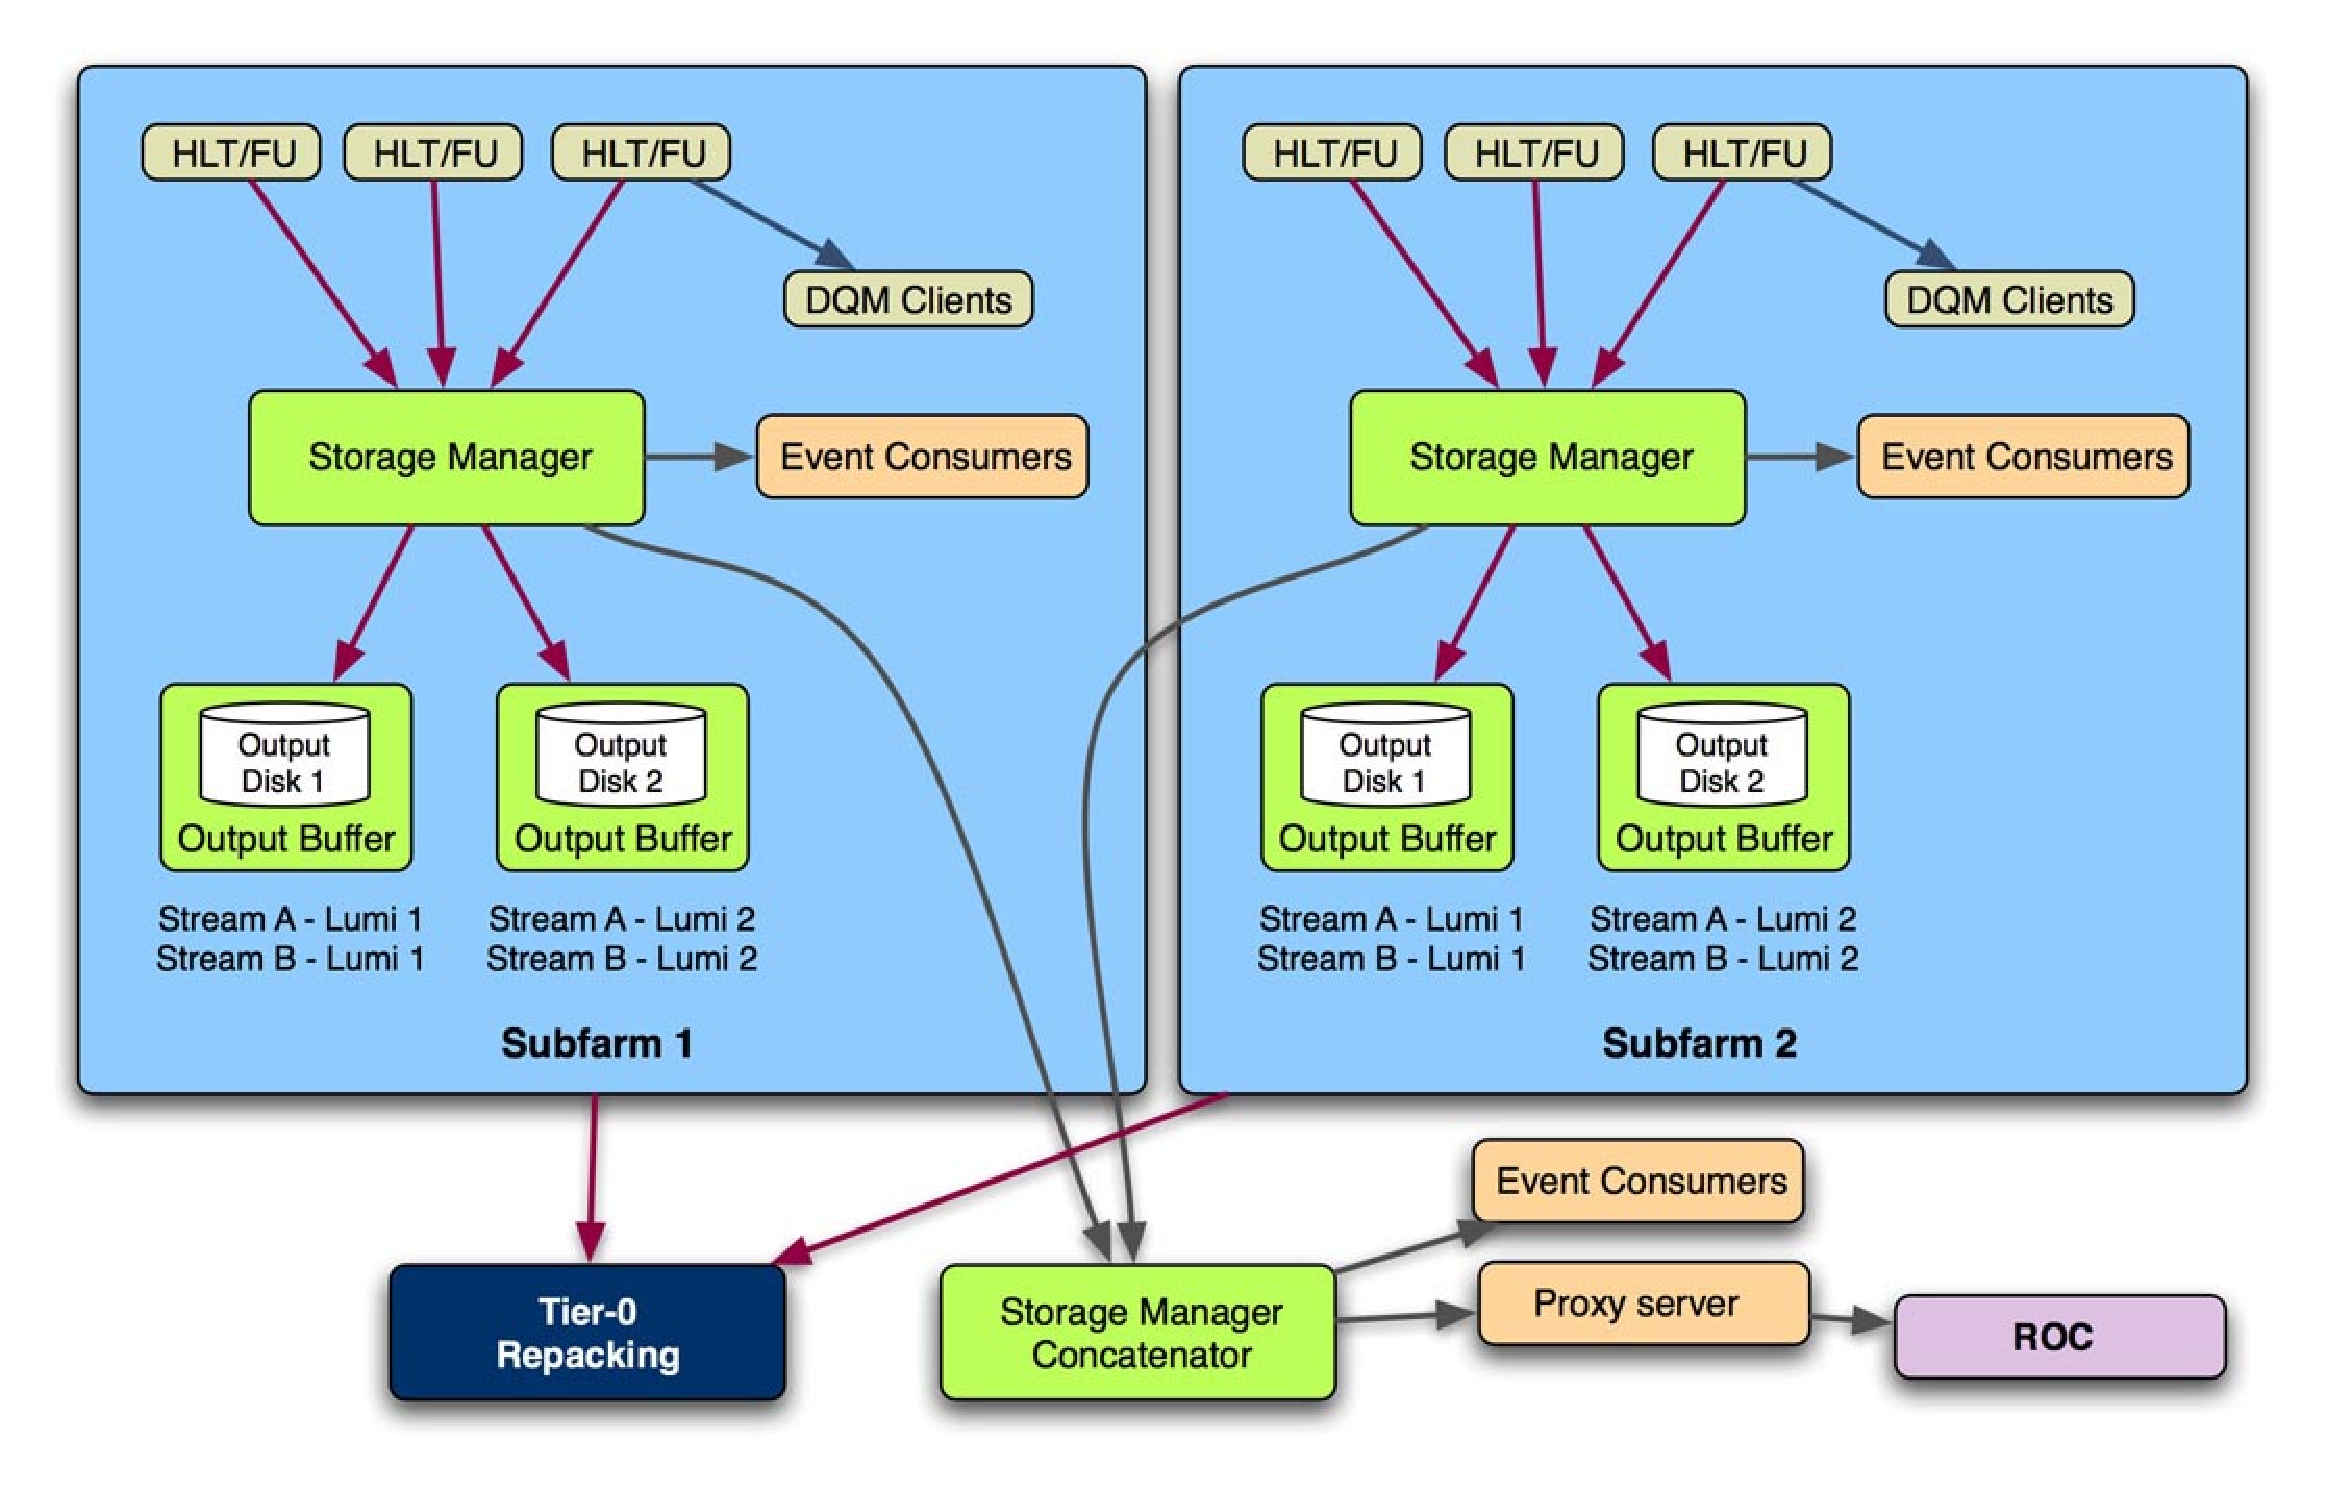
\includegraphics[width=5.5in]{SM_architecture_base.eps}
    \caption{Base design.}
    \label{fig:base_design}
  \end{center}
\end{figure}

\subsubsection{Implementation Details}

\begin{figure}[hbtp]
  \begin{center}
    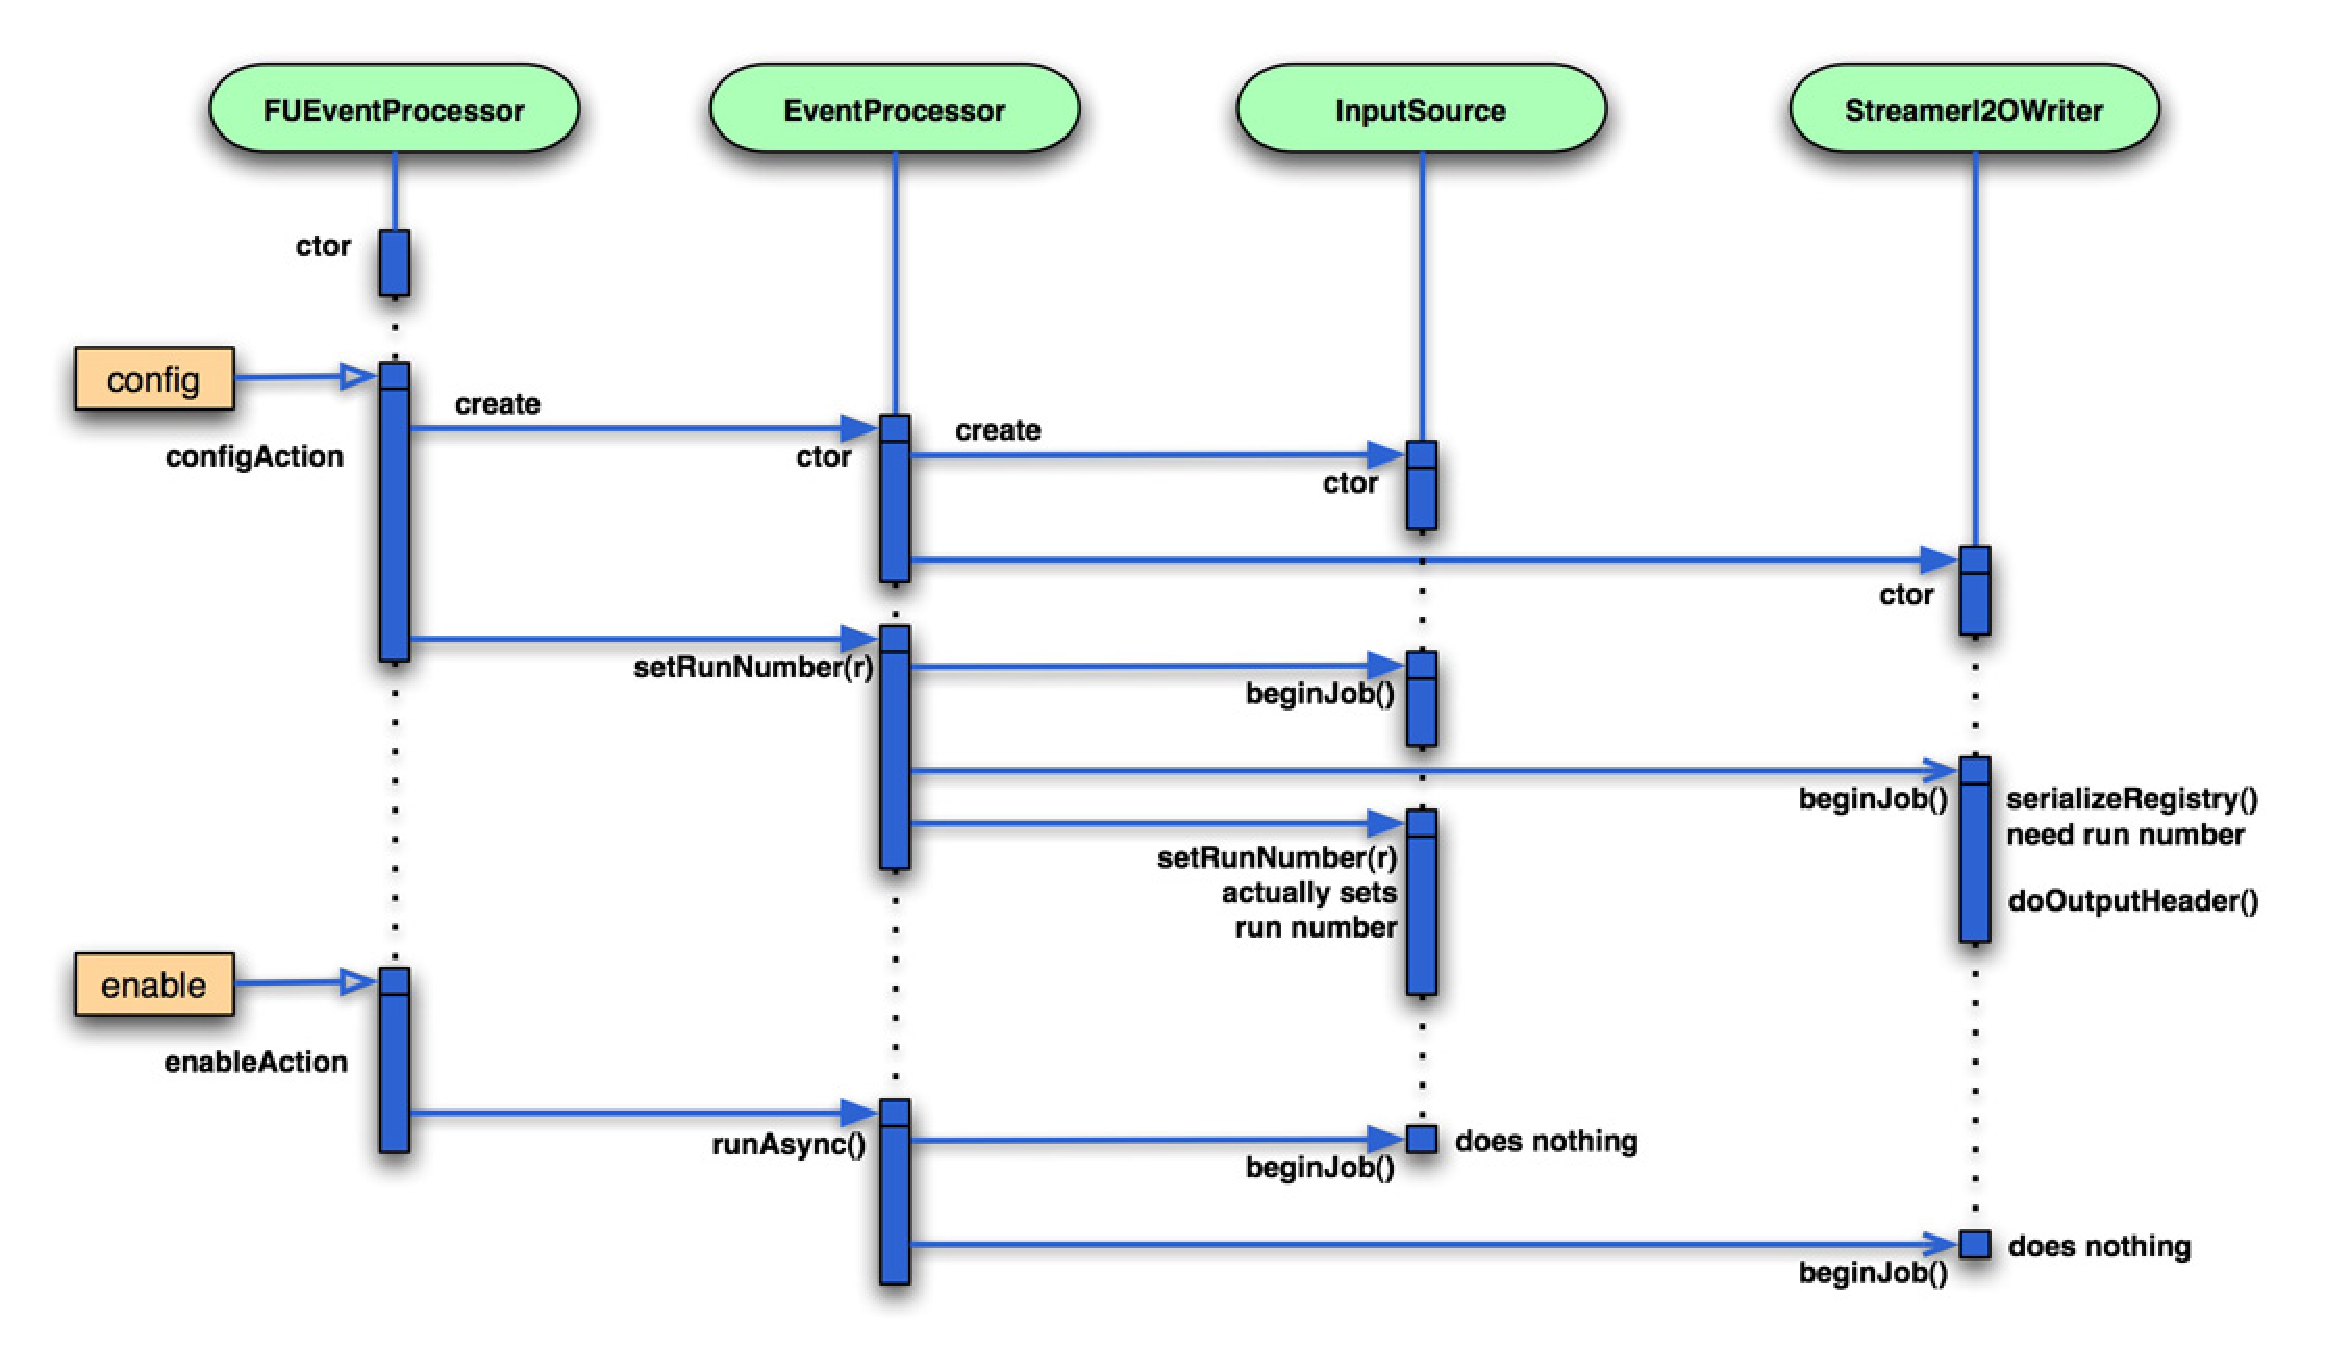
\includegraphics[width=5.5in]{SM_base_code1_prt-2.eps}
    \caption{FUEventProcessor call sequence for setting the run number.}
    \label{fig:base_FUEP_code}
  \end{center}
\end{figure}

\begin{figure}[hbtp]
  \begin{center}
    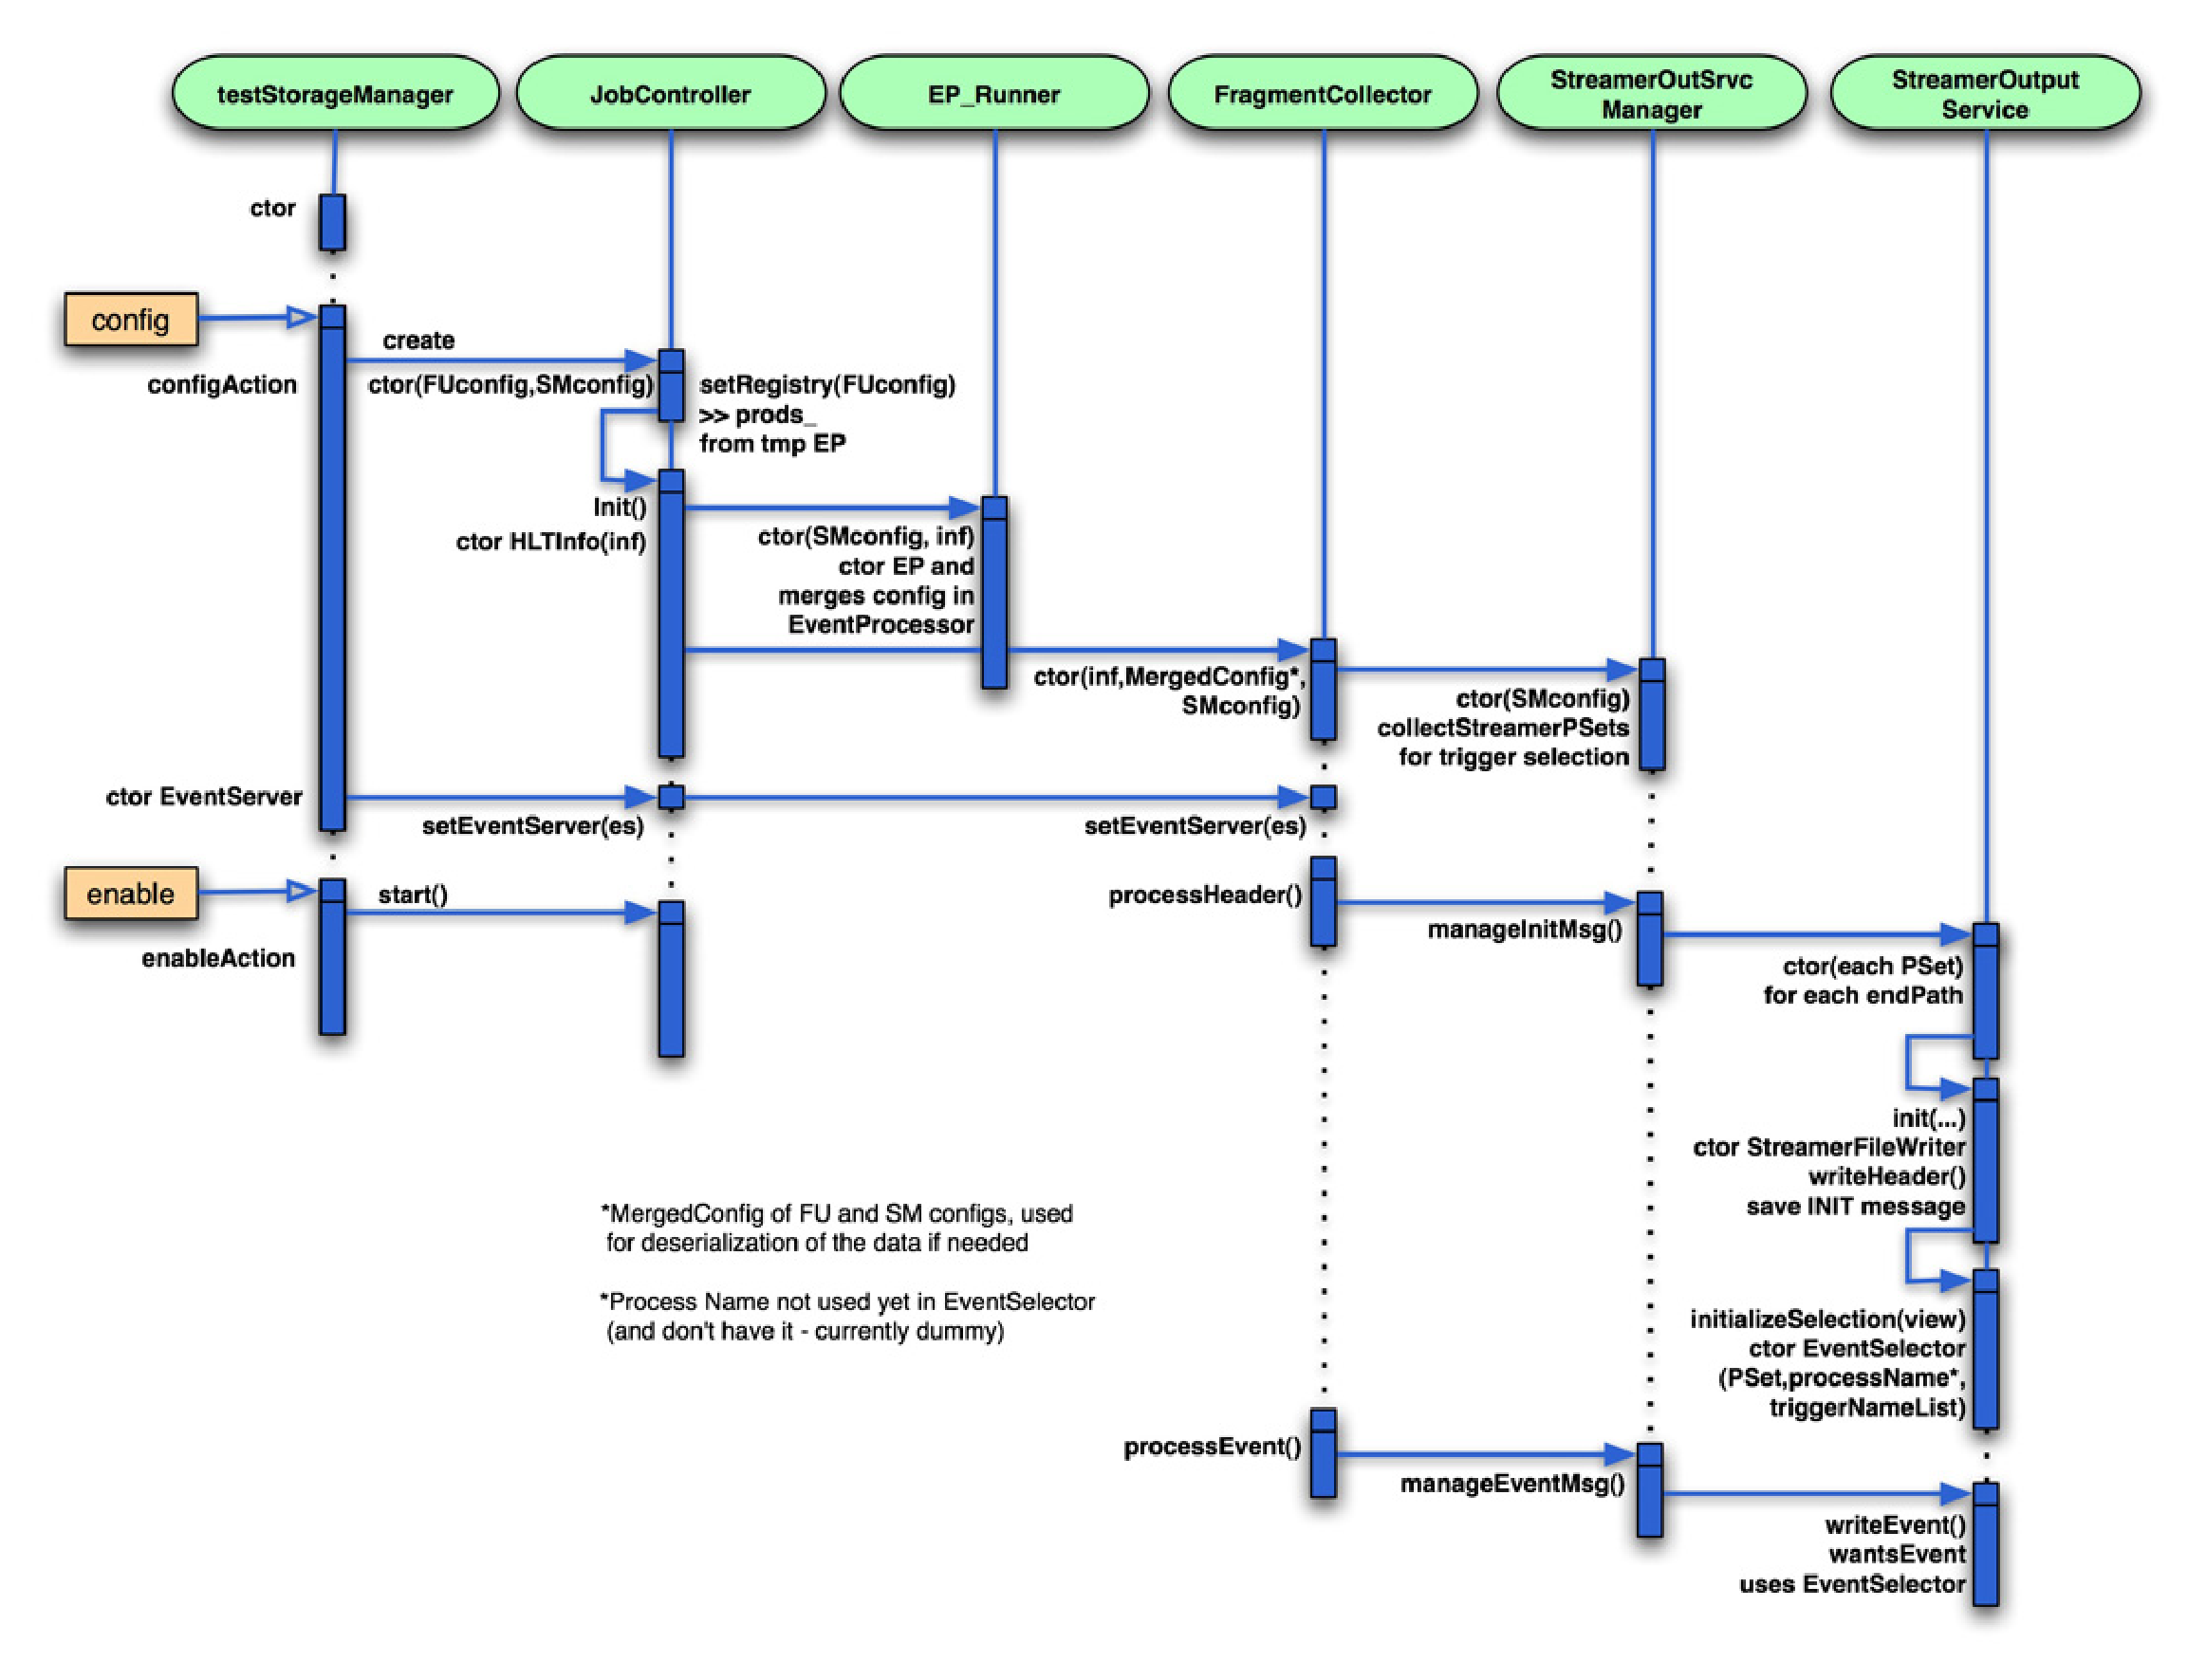
\includegraphics[width=5.5in]{SM_base_code2_prt-2.eps}
    \caption{Storage Manager configuration sequence.}
    \label{fig:base_SMCF_code}
  \end{center}
\end{figure}

\begin{figure}[hbtp]
  \begin{center}
    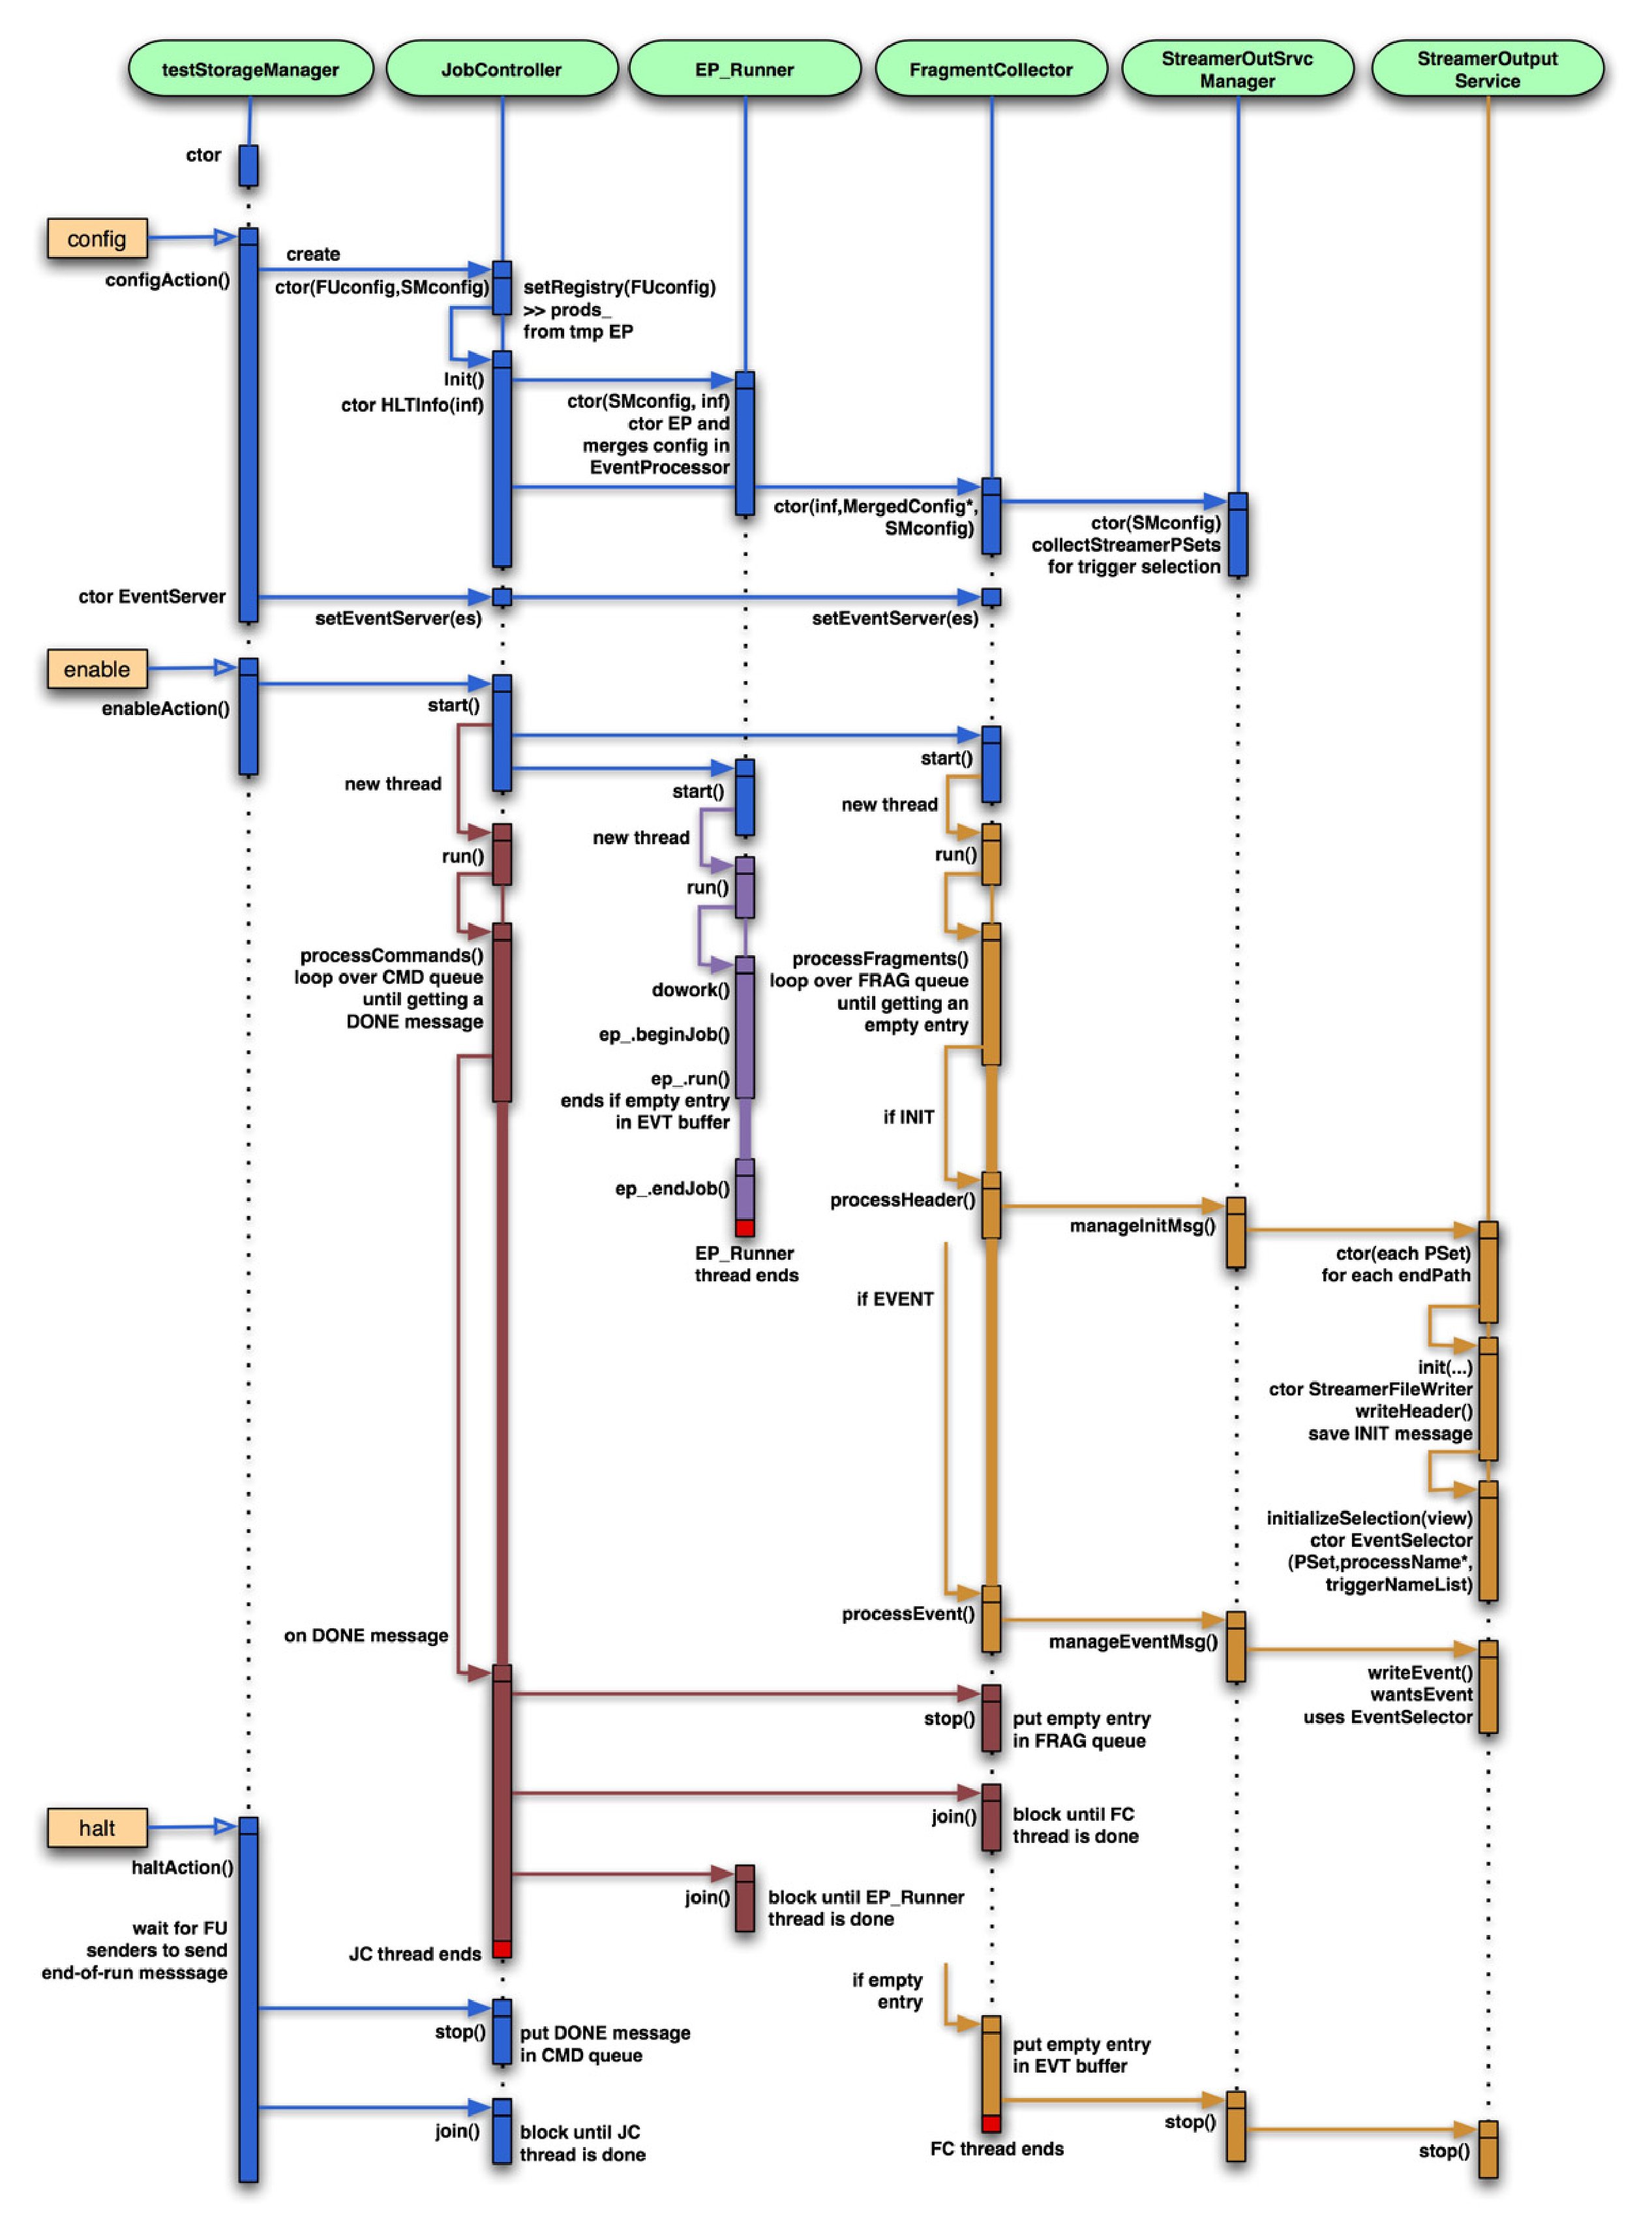
\includegraphics[width=6.0in]{SM_base_code3_prt-2.eps}
    \caption{Storage Manager sequence for prototype 2 code used in
    MTCC phase 2.}
    \label{fig:base_SMMTCC_code}
  \end{center}
\end{figure}

\begin{figure}[hbtp]
  \begin{center}
    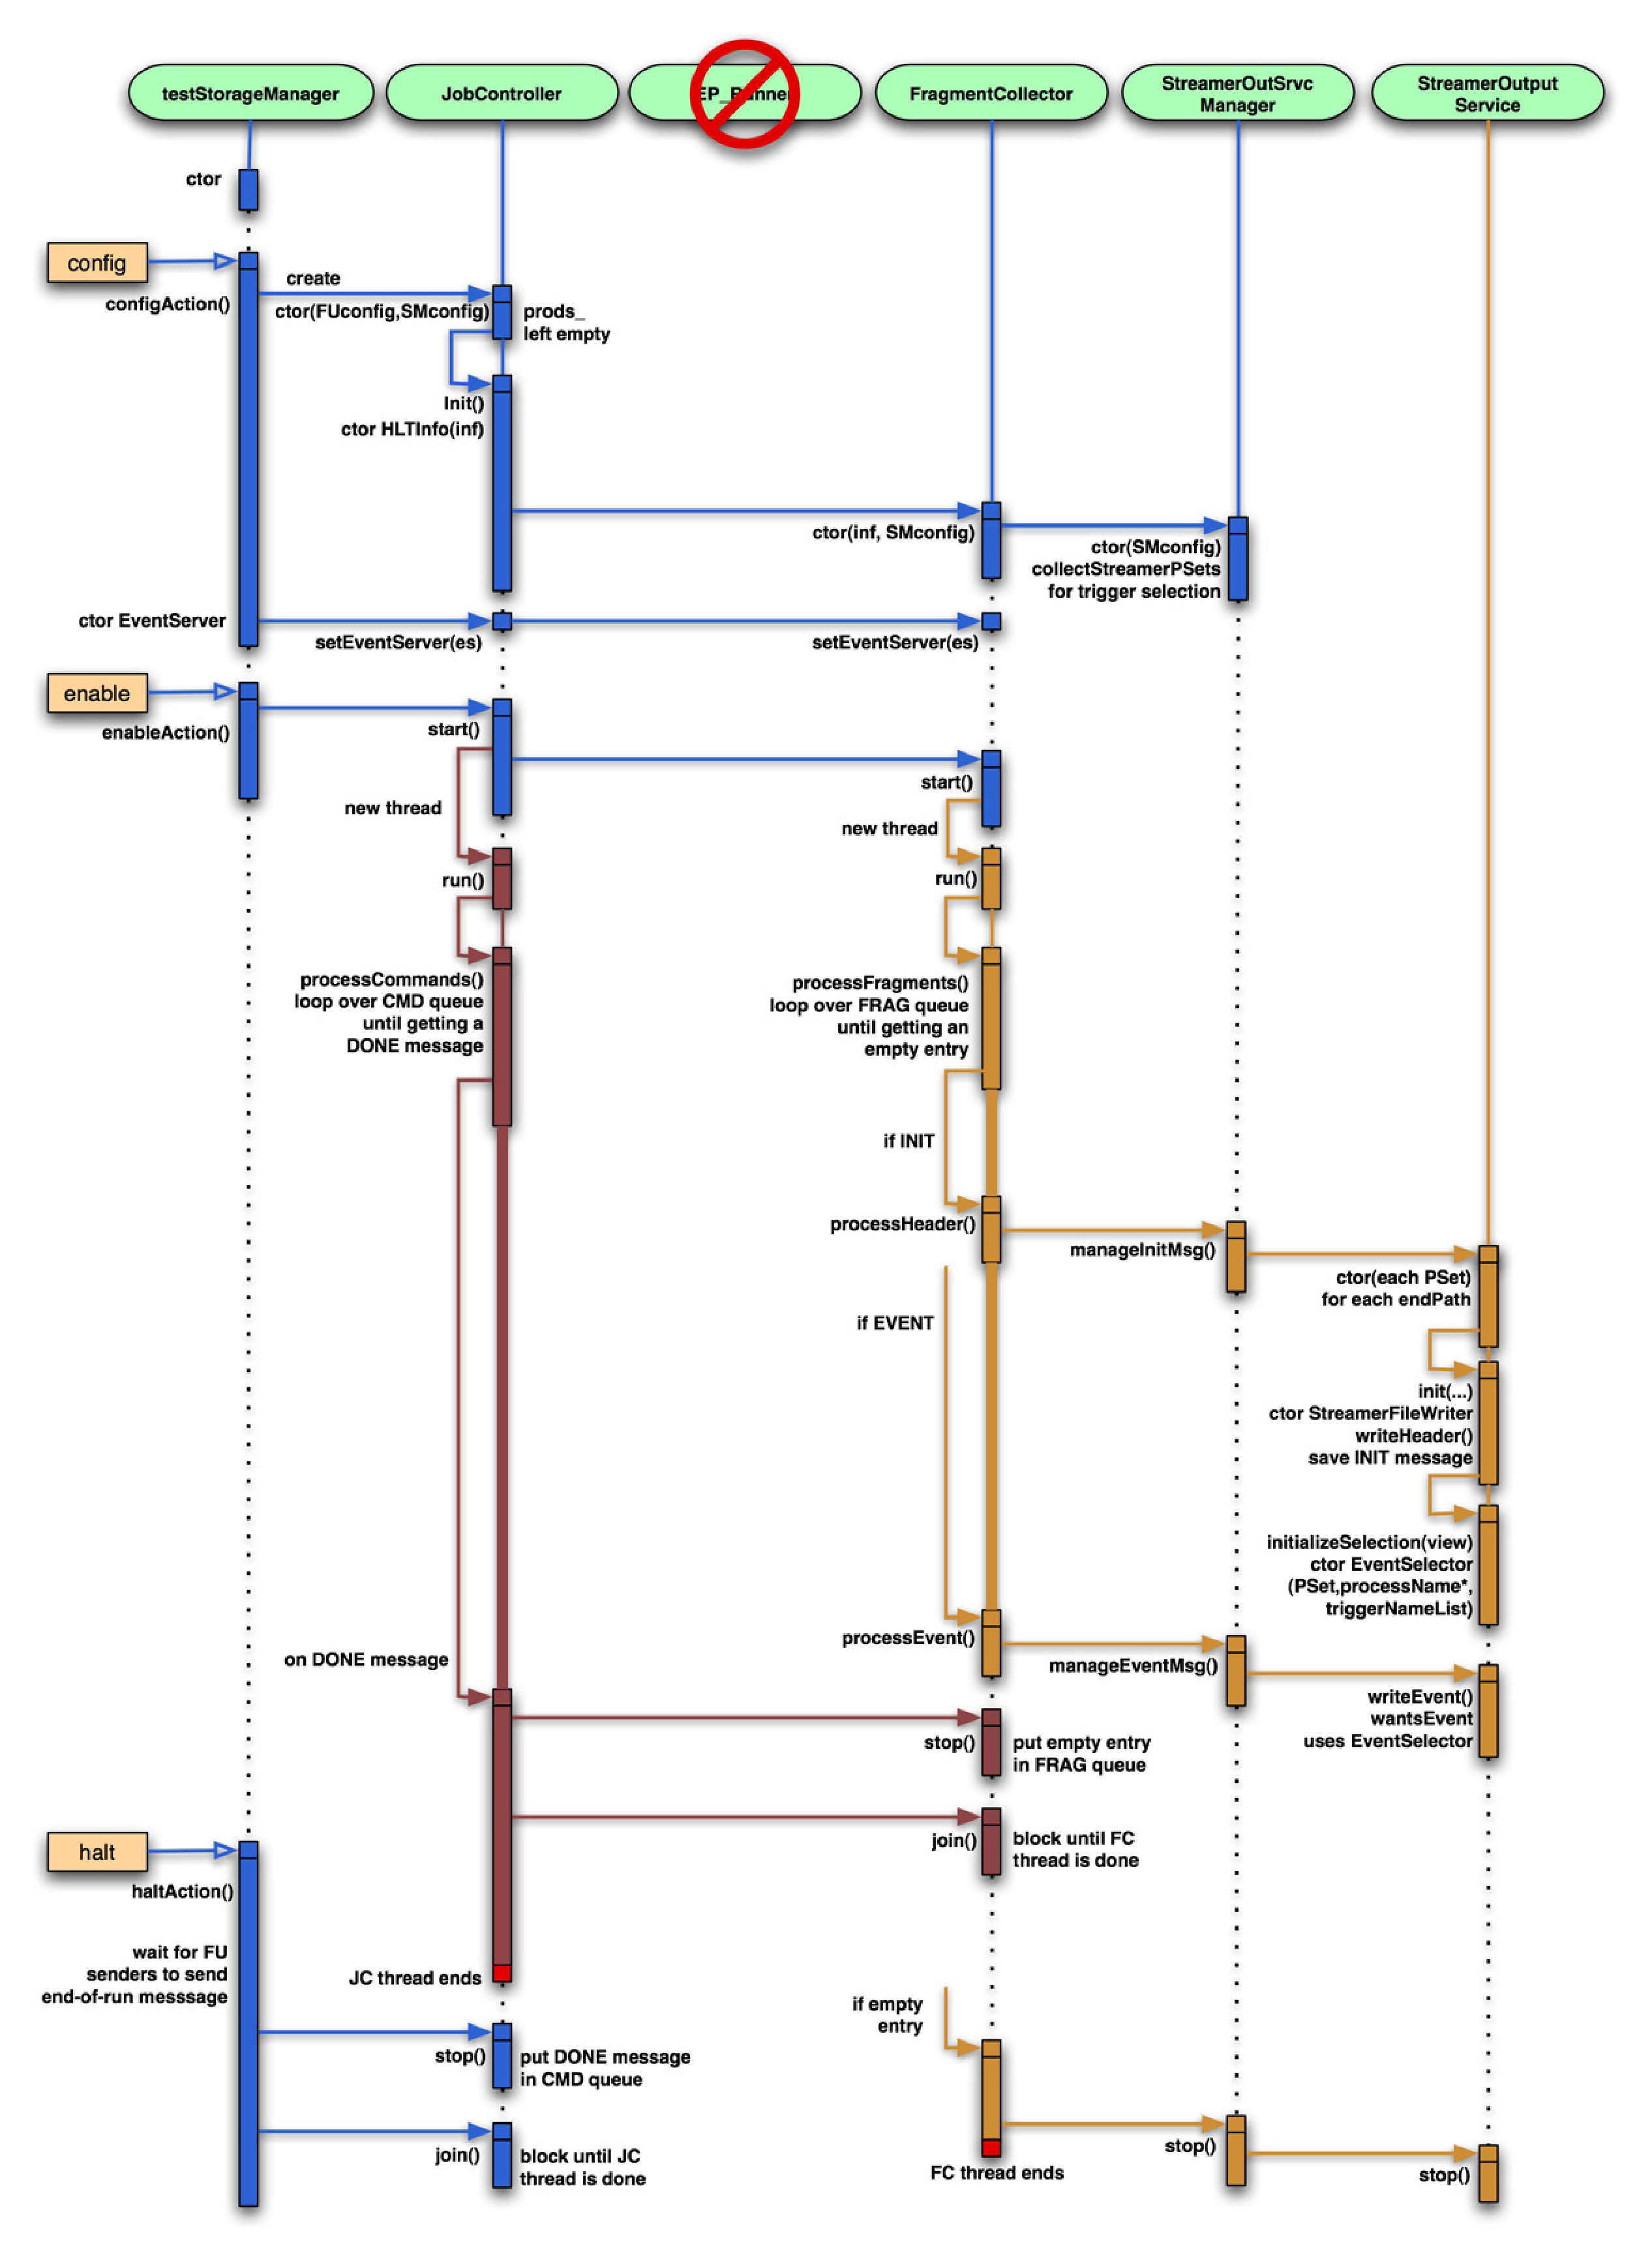
\includegraphics[width=6.0in]{SM_prd_code3_prt-2.eps}
    \caption{Storage Manager sequence for production code.}
    \label{fig:base_SMPRD_code}
  \end{center}
\end{figure}


\subsubsection{Possible Extension}

\begin{figure}[hbtp]
  \begin{center}
    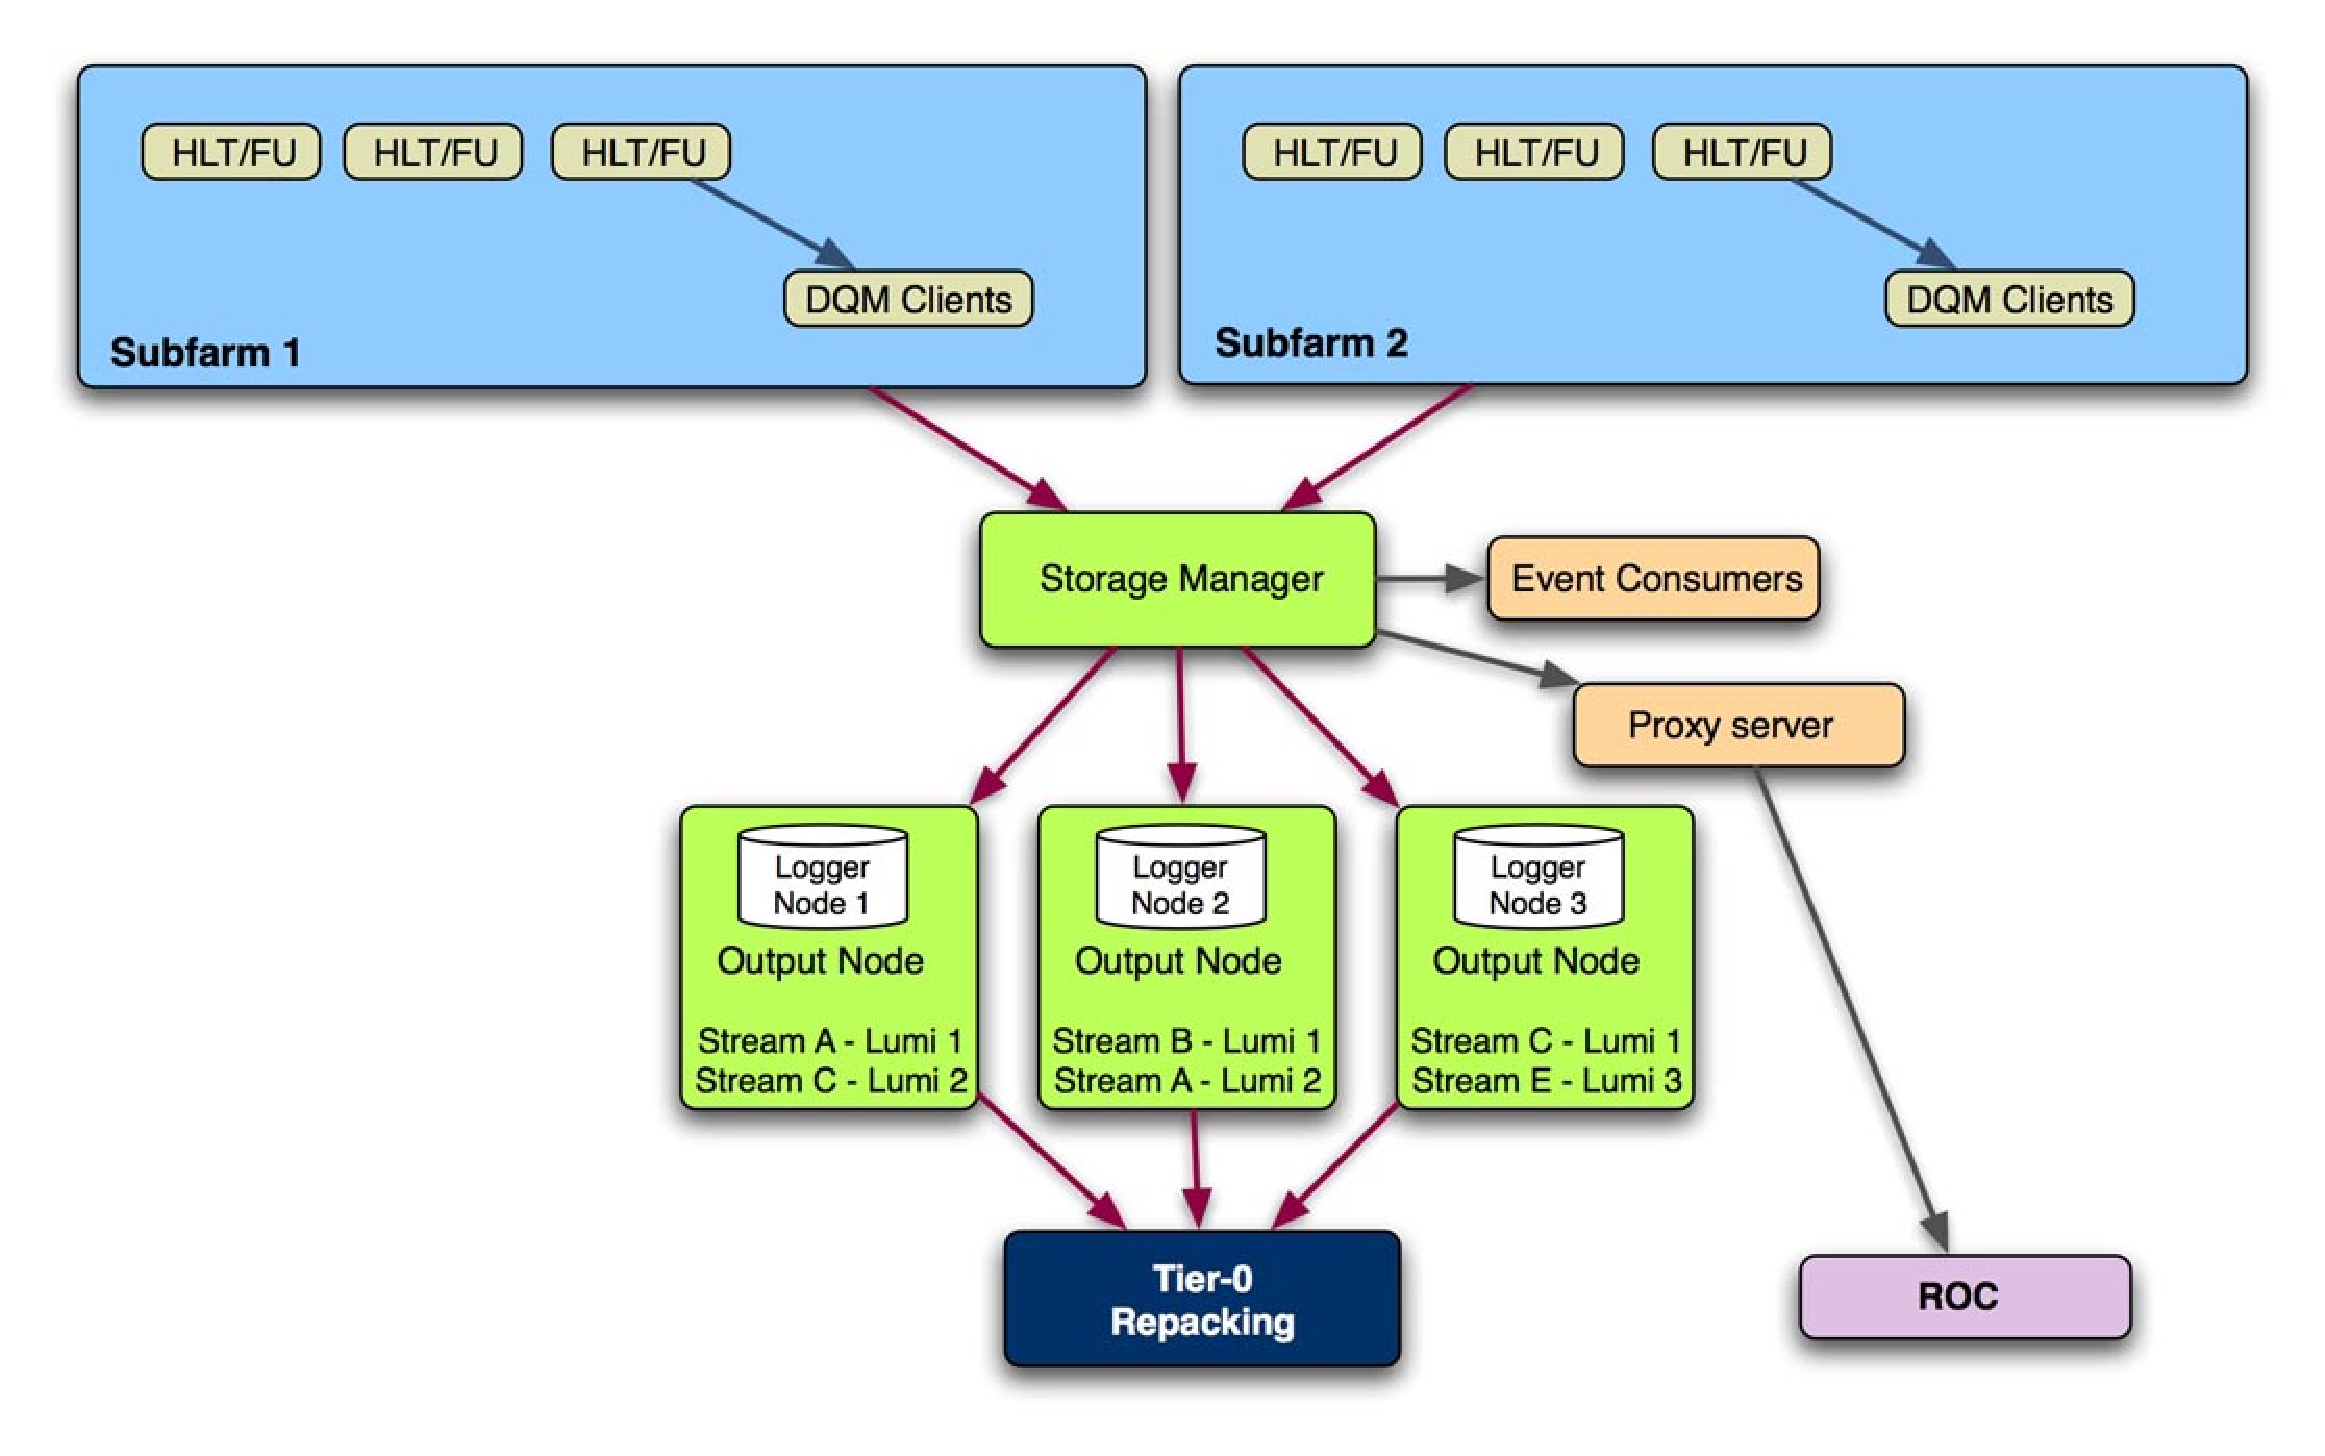
\includegraphics[width=5.5in]{SM_architecture_opt1.eps}
    \caption{Base design with integrated concatenator.}
    \label{fig:opt1_design}
  \end{center}
\end{figure}


\subsubsection{Future Design}

\begin{figure}[hbtp]
  \begin{center}
    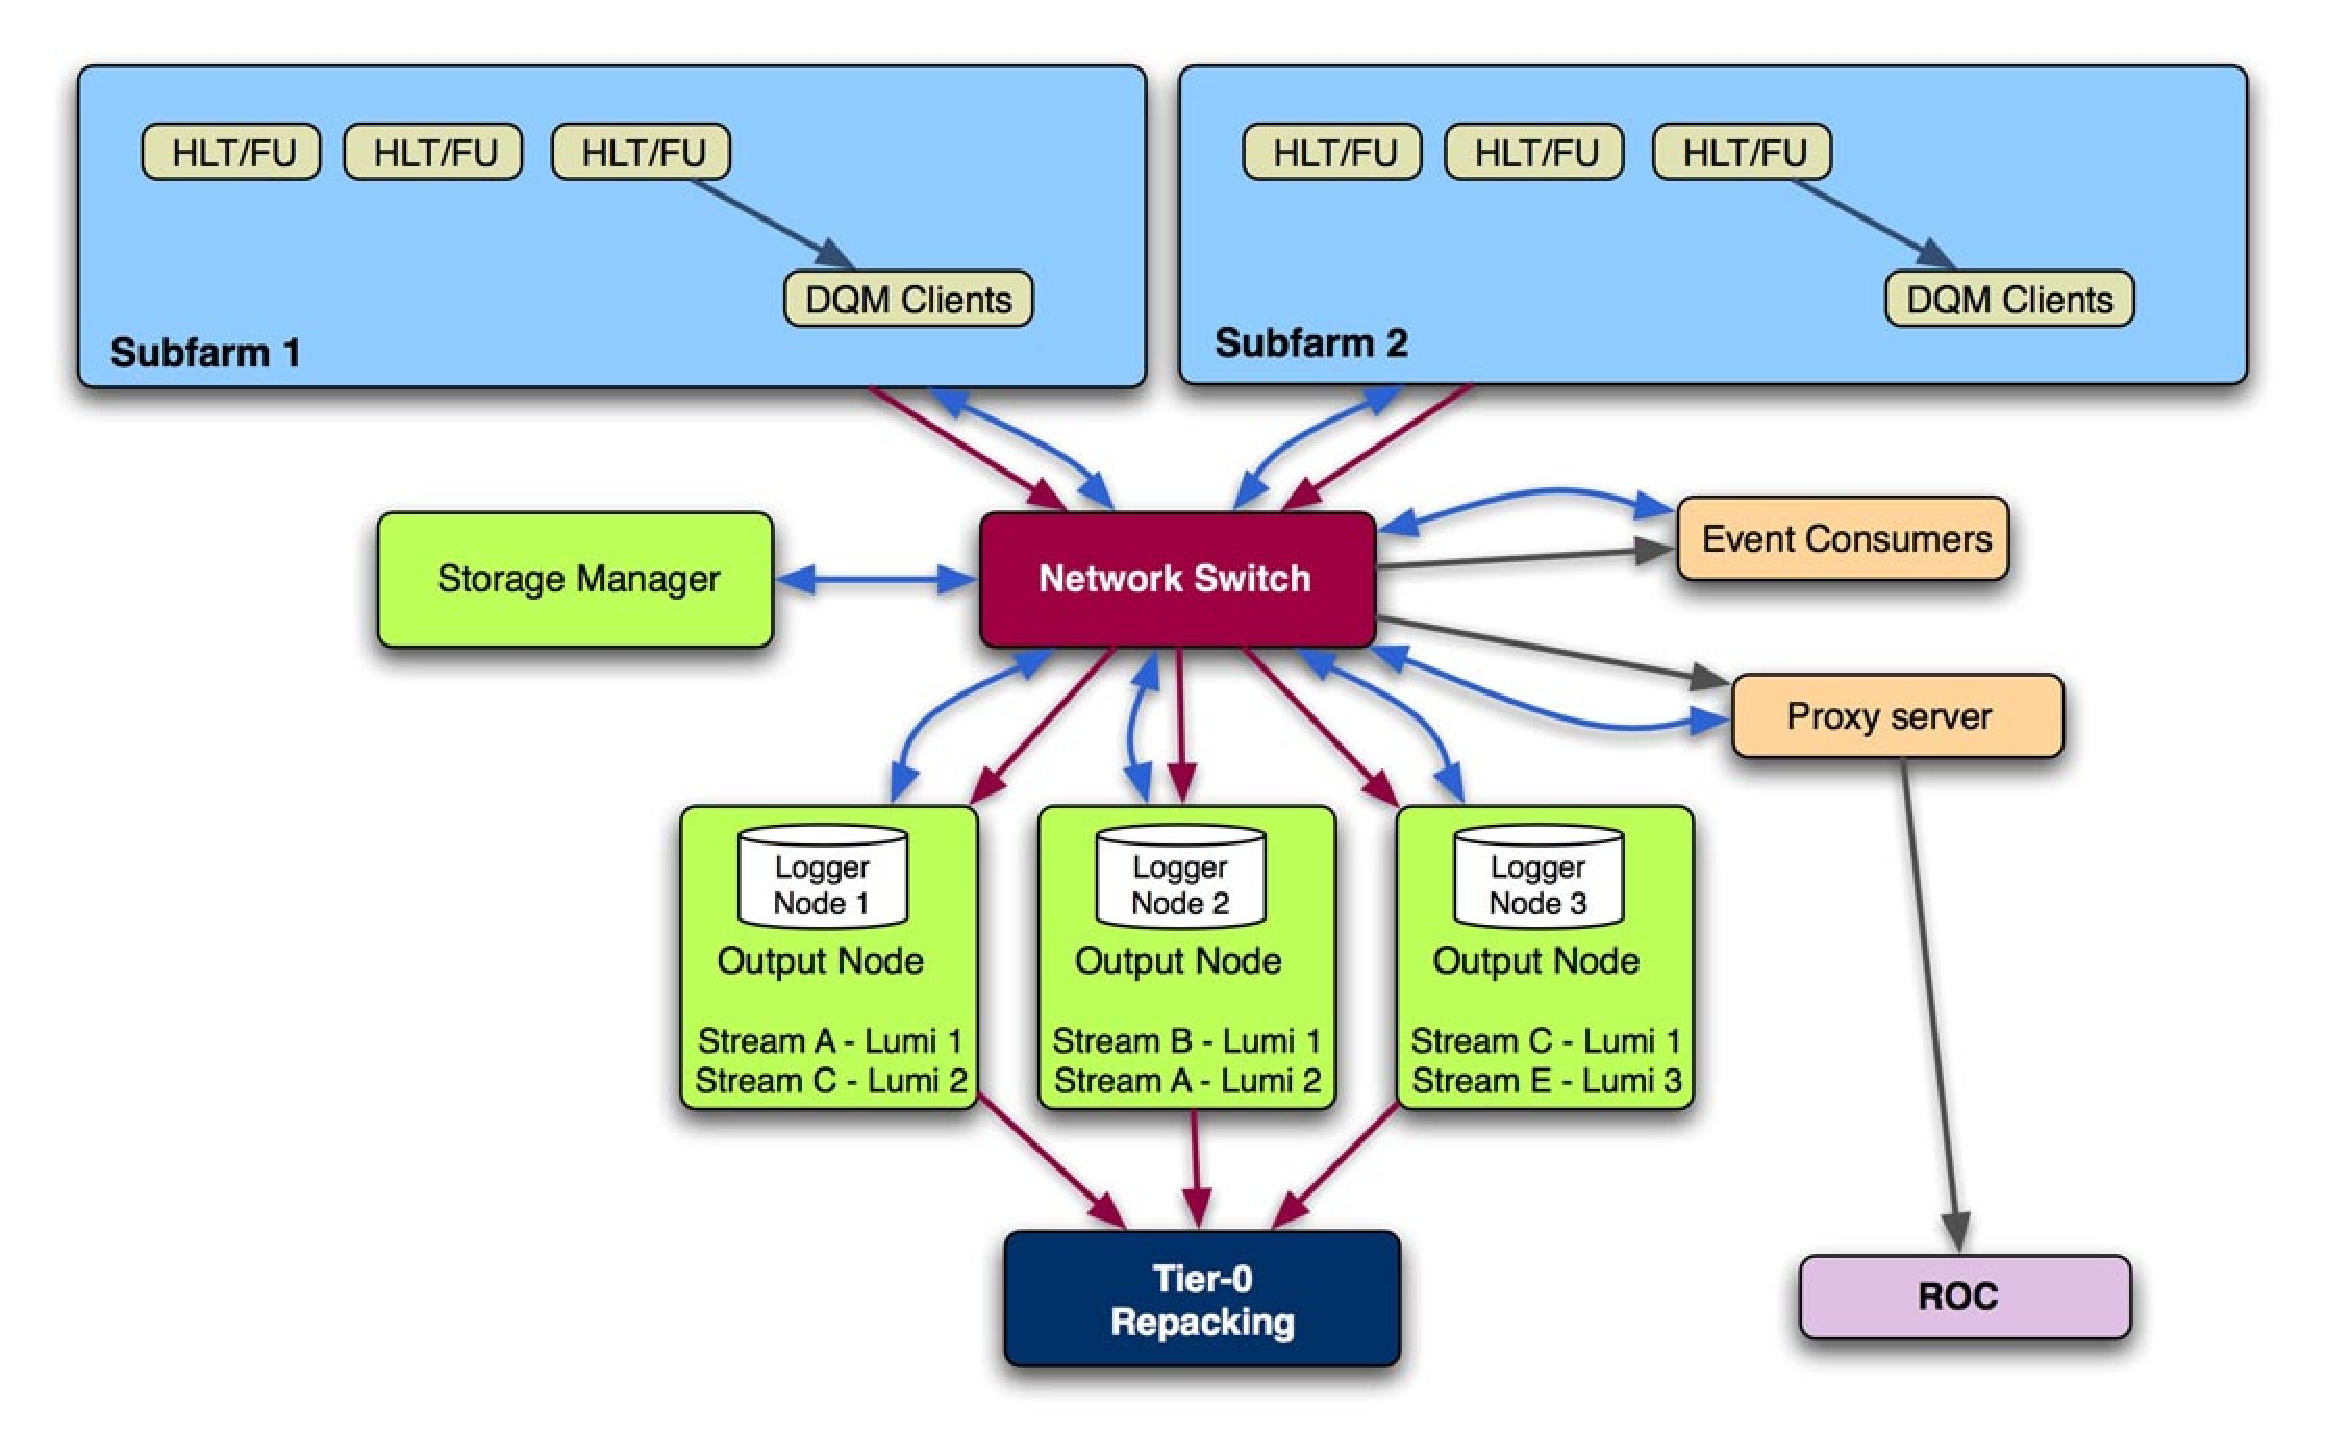
\includegraphics[width=5.5in]{SM_architecture_opt2.eps}
    \caption{Distributed Design.}
    \label{fig:opt2_design}
  \end{center}
\end{figure}

\subsubsection{Interaction with Tier-0}

\subsubsection{Interaction with Run Control}

Include DQM (hot disks, caches?)


\subsection{Communication and Output}

\subsubsection{Application protocol}

\flushleft{\bf Event Filter Unit (message formats)}

\flushleft{\bf Run Control}

\flushleft{\bf Tier-0}

\subsubsection{File formats}

Include index file

\subsection{Functions and Implementation}

\subsubsection{FU Output module}

\subsubsection{SM Input module and Collector}

\subsubsection{Internal event processing}

\subsubsection{SM Output module}

\subsubsection{Event Server Manager}

\subsubsection{Monitoring, Statistics and Book-keeping}


\section{External Functions and Interaction}

\subsection{Interaction with Databases}

\subsection{File and Disk Management Application}

Functions and design of the script(s).

\subsubsection{Conversion}

\subsubsection{Monitoring and Statistics}

Include trigger rates

%\documentclass{article}
\documentclass[landscape]{article}
\usepackage{amsmath,pennames}

\newif\ifpdf
\ifx\pdfoutput\undefined
 \pdffalse
\else
 \pdftrue
\fi

\pdffalse

\ifpdf
 \usepackage[pdftex]{color}
 \usepackage[pdftex]{graphicx}
 \usepackage[pdftex,bookmarks=true,bookmarksopen=true]{hyperref}
\else
 \usepackage{color}
 \usepackage{graphicx}
 \usepackage{hyperref}
\fi



\addtolength{\topmargin}{-1.0in}
\addtolength{\textheight}{2.0in}

\addtolength{\textwidth}{2.0in}
\addtolength{\oddsidemargin}{-1.0in}
\addtolength{\evensidemargin}{1.0in}

%%%%%%%%%%%%%%%%%%%%%%%%%%%%%%%%%%%%%%%%%%%%%%%%%%%%%%%%%%%%%%%%%%%%%%%%%%%%%%%
\begin{document}

\section{ppPixel}

\subsection{Geometrical acceptance}
 \includegraphics[width=0.5\textwidth]{../eps/ppPixel/geomAccepEta}
 \includegraphics[width=0.5\textwidth]{../eps/ppPixel/geomAccepPt}
 \includegraphics[width=0.5\textwidth]{../eps/ppPixel/geomAccepEtaPt_pion}
 \includegraphics[width=0.5\textwidth]{../eps/ppPixel/geomAccepLogPt}
%\includegraphics[width=0.5\textwidth]{../eps/ppPixel/geomAccepEtaPt_kaon}
%\includegraphics[width=0.5\textwidth]{../eps/ppPixel/geomAccepEtaPt_prot}
 \newpage
 
\subsection{Algorithmic efficiency}
 \includegraphics[width=0.5\textwidth]{../eps/ppPixel/algoEfficEta}
 \includegraphics[width=0.5\textwidth]{../eps/ppPixel/algoEfficPt}
 \includegraphics[width=0.5\textwidth]{../eps/ppPixel/algoEfficEtaPt_pion}
 \includegraphics[width=0.5\textwidth]{../eps/ppPixel/algoEfficLogPt}
%\includegraphics[width=0.5\textwidth]{../eps/ppPixel/algoEfficEtaPt_kaon}
%\includegraphics[width=0.5\textwidth]{../eps/ppPixel/algoEfficEtaPt_prot}
 \newpage

\subsection{Multiple counting}
 \includegraphics[width=0.5\textwidth]{../eps/ppPixel/multCountEta}
 \includegraphics[width=0.5\textwidth]{../eps/ppPixel/multCountPt}
 \includegraphics[width=0.5\textwidth]{../eps/ppPixel/multCountEtaPt_pion}
 \includegraphics[width=0.5\textwidth]{../eps/ppPixel/multCountLogPt}
%\includegraphics[width=0.5\textwidth]{../eps/ppPixel/multCountEtaPt_kaon}
%\includegraphics[width=0.5\textwidth]{../eps/ppPixel/multCountEtaPt_prot}
 \newpage

\subsection{Fake track rate}
 \includegraphics[width=0.5\textwidth]{../eps/ppPixel/fakeRateEta}
 \includegraphics[width=0.5\textwidth]{../eps/ppPixel/fakeRatePt}
 \includegraphics[width=0.5\textwidth]{../eps/ppPixel/fakeRateEtaPt}
 \includegraphics[width=0.5\textwidth]{../eps/ppPixel/fakeRateLogPt}
 \newpage

\subsection{Bias and resolution}
 \includegraphics[width=0.5\textwidth]{../eps/ppPixel/ptBias}
 \includegraphics[width=0.5\textwidth]{../eps/ppPixel/ptReso}
 \rightline{
 \includegraphics[width=0.5\textwidth]{../eps/ppPixel/ptLogReso}}
%\includegraphics[width=0.5\textwidth]{../eps/ppPixel/ptBias}
%\includegraphics[width=0.5\textwidth]{../eps/ppPixel/ptReso}
%\includegraphics[width=0.5\textwidth]{../eps/ppPixel/ptBiar}
%\includegraphics[width=0.5\textwidth]{../eps/ppPixel/ptResr}
 \newpage
\section{ppGlobal}

\subsection{Geometrical acceptance}
 \includegraphics[width=0.5\textwidth]{../eps/ppGlobal/geomAccepEta}
 \includegraphics[width=0.5\textwidth]{../eps/ppGlobal/geomAccepPt}
 \includegraphics[width=0.5\textwidth]{../eps/ppGlobal/geomAccepEtaPt_pion}
 \includegraphics[width=0.5\textwidth]{../eps/ppGlobal/geomAccepLogPt}
%\includegraphics[width=0.5\textwidth]{../eps/ppGlobal/geomAccepEtaPt_kaon}
%\includegraphics[width=0.5\textwidth]{../eps/ppGlobal/geomAccepEtaPt_prot}
 \newpage
 
\subsection{Algorithmic efficiency}
 \includegraphics[width=0.5\textwidth]{../eps/ppGlobal/algoEfficEta}
 \includegraphics[width=0.5\textwidth]{../eps/ppGlobal/algoEfficPt}
 \includegraphics[width=0.5\textwidth]{../eps/ppGlobal/algoEfficEtaPt_pion}
 \includegraphics[width=0.5\textwidth]{../eps/ppGlobal/algoEfficLogPt}
%\includegraphics[width=0.5\textwidth]{../eps/ppGlobal/algoEfficEtaPt_kaon}
%\includegraphics[width=0.5\textwidth]{../eps/ppGlobal/algoEfficEtaPt_prot}
 \newpage

\subsection{Multiple counting}
 \includegraphics[width=0.5\textwidth]{../eps/ppGlobal/multCountEta}
 \includegraphics[width=0.5\textwidth]{../eps/ppGlobal/multCountPt}
 \includegraphics[width=0.5\textwidth]{../eps/ppGlobal/multCountEtaPt_pion}
 \includegraphics[width=0.5\textwidth]{../eps/ppGlobal/multCountLogPt}
%\includegraphics[width=0.5\textwidth]{../eps/ppGlobal/multCountEtaPt_kaon}
%\includegraphics[width=0.5\textwidth]{../eps/ppGlobal/multCountEtaPt_prot}
 \newpage

\subsection{Fake track rate}
 \includegraphics[width=0.5\textwidth]{../eps/ppGlobal/fakeRateEta}
 \includegraphics[width=0.5\textwidth]{../eps/ppGlobal/fakeRatePt}
 \includegraphics[width=0.5\textwidth]{../eps/ppGlobal/fakeRateEtaPt}
 \includegraphics[width=0.5\textwidth]{../eps/ppGlobal/fakeRateLogPt}
 \newpage

\subsection{Bias and resolution}
 \includegraphics[width=0.5\textwidth]{../eps/ppGlobal/ptBias}
 \includegraphics[width=0.5\textwidth]{../eps/ppGlobal/ptReso}
 \rightline{
 \includegraphics[width=0.5\textwidth]{../eps/ppGlobal/ptLogReso}}
%\includegraphics[width=0.5\textwidth]{../eps/ppGlobal/ptBias}
%\includegraphics[width=0.5\textwidth]{../eps/ppGlobal/ptReso}
%\includegraphics[width=0.5\textwidth]{../eps/ppGlobal/ptBiar}
%\includegraphics[width=0.5\textwidth]{../eps/ppGlobal/ptResr}
 \newpage
\section{PbPbPixel}

\subsection{Geometrical acceptance}
 \includegraphics[width=0.5\textwidth]{../eps/PbPbPixel/geomAccepEta}
 \includegraphics[width=0.5\textwidth]{../eps/PbPbPixel/geomAccepPt}
 \includegraphics[width=0.5\textwidth]{../eps/PbPbPixel/geomAccepEtaPt_pion}
 \includegraphics[width=0.5\textwidth]{../eps/PbPbPixel/geomAccepLogPt}
%\includegraphics[width=0.5\textwidth]{../eps/PbPbPixel/geomAccepEtaPt_kaon}
%\includegraphics[width=0.5\textwidth]{../eps/PbPbPixel/geomAccepEtaPt_prot}
 \newpage
 
\subsection{Algorithmic efficiency}
 \includegraphics[width=0.5\textwidth]{../eps/PbPbPixel/algoEfficEta}
 \includegraphics[width=0.5\textwidth]{../eps/PbPbPixel/algoEfficPt}
 \includegraphics[width=0.5\textwidth]{../eps/PbPbPixel/algoEfficEtaPt_pion}
 \includegraphics[width=0.5\textwidth]{../eps/PbPbPixel/algoEfficLogPt}
%\includegraphics[width=0.5\textwidth]{../eps/PbPbPixel/algoEfficEtaPt_kaon}
%\includegraphics[width=0.5\textwidth]{../eps/PbPbPixel/algoEfficEtaPt_prot}
 \newpage

\subsection{Multiple counting}
 \includegraphics[width=0.5\textwidth]{../eps/PbPbPixel/multCountEta}
 \includegraphics[width=0.5\textwidth]{../eps/PbPbPixel/multCountPt}
 \includegraphics[width=0.5\textwidth]{../eps/PbPbPixel/multCountEtaPt_pion}
 \includegraphics[width=0.5\textwidth]{../eps/PbPbPixel/multCountLogPt}
%\includegraphics[width=0.5\textwidth]{../eps/PbPbPixel/multCountEtaPt_kaon}
%\includegraphics[width=0.5\textwidth]{../eps/PbPbPixel/multCountEtaPt_prot}
 \newpage

\subsection{Fake track rate}
 \includegraphics[width=0.5\textwidth]{../eps/PbPbPixel/fakeRateEta}
 \includegraphics[width=0.5\textwidth]{../eps/PbPbPixel/fakeRatePt}
 \includegraphics[width=0.5\textwidth]{../eps/PbPbPixel/fakeRateEtaPt}
 \includegraphics[width=0.5\textwidth]{../eps/PbPbPixel/fakeRateLogPt}
 \newpage

\subsection{Bias and resolution}
 \includegraphics[width=0.5\textwidth]{../eps/PbPbPixel/ptBias}
 \includegraphics[width=0.5\textwidth]{../eps/PbPbPixel/ptReso}
 \rightline{
 \includegraphics[width=0.5\textwidth]{../eps/PbPbPixel/ptLogReso}}
%\includegraphics[width=0.5\textwidth]{../eps/PbPbPixel/ptBias}
%\includegraphics[width=0.5\textwidth]{../eps/PbPbPixel/ptReso}
%\includegraphics[width=0.5\textwidth]{../eps/PbPbPixel/ptBiar}
%\includegraphics[width=0.5\textwidth]{../eps/PbPbPixel/ptResr}
 \newpage
\section{PbPbGlobal}

\subsection{Geometrical acceptance}
 \includegraphics[width=0.5\textwidth]{../eps/PbPbGlobal/geomAccepEta}
 \includegraphics[width=0.5\textwidth]{../eps/PbPbGlobal/geomAccepPt}
 \includegraphics[width=0.5\textwidth]{../eps/PbPbGlobal/geomAccepEtaPt_pion}
 \includegraphics[width=0.5\textwidth]{../eps/PbPbGlobal/geomAccepLogPt}
%\includegraphics[width=0.5\textwidth]{../eps/PbPbGlobal/geomAccepEtaPt_kaon}
%\includegraphics[width=0.5\textwidth]{../eps/PbPbGlobal/geomAccepEtaPt_prot}
 \newpage
 
\subsection{Algorithmic efficiency}
 \includegraphics[width=0.5\textwidth]{../eps/PbPbGlobal/algoEfficEta}
 \includegraphics[width=0.5\textwidth]{../eps/PbPbGlobal/algoEfficPt}
 \includegraphics[width=0.5\textwidth]{../eps/PbPbGlobal/algoEfficEtaPt_pion}
 \includegraphics[width=0.5\textwidth]{../eps/PbPbGlobal/algoEfficLogPt}
%\includegraphics[width=0.5\textwidth]{../eps/PbPbGlobal/algoEfficEtaPt_kaon}
%\includegraphics[width=0.5\textwidth]{../eps/PbPbGlobal/algoEfficEtaPt_prot}
 \newpage

\subsection{Multiple counting}
 \includegraphics[width=0.5\textwidth]{../eps/PbPbGlobal/multCountEta}
 \includegraphics[width=0.5\textwidth]{../eps/PbPbGlobal/multCountPt}
 \includegraphics[width=0.5\textwidth]{../eps/PbPbGlobal/multCountEtaPt_pion}
 \includegraphics[width=0.5\textwidth]{../eps/PbPbGlobal/multCountLogPt}
%\includegraphics[width=0.5\textwidth]{../eps/PbPbGlobal/multCountEtaPt_kaon}
%\includegraphics[width=0.5\textwidth]{../eps/PbPbGlobal/multCountEtaPt_prot}
 \newpage

\subsection{Fake track rate}
 \includegraphics[width=0.5\textwidth]{../eps/PbPbGlobal/fakeRateEta}
 \includegraphics[width=0.5\textwidth]{../eps/PbPbGlobal/fakeRatePt}
 \includegraphics[width=0.5\textwidth]{../eps/PbPbGlobal/fakeRateEtaPt}
 \includegraphics[width=0.5\textwidth]{../eps/PbPbGlobal/fakeRateLogPt}
 \newpage

\subsection{Bias and resolution}
 \includegraphics[width=0.5\textwidth]{../eps/PbPbGlobal/ptBias}
 \includegraphics[width=0.5\textwidth]{../eps/PbPbGlobal/ptReso}
 \rightline{
 \includegraphics[width=0.5\textwidth]{../eps/PbPbGlobal/ptLogReso}}
%\includegraphics[width=0.5\textwidth]{../eps/PbPbGlobal/ptBias}
%\includegraphics[width=0.5\textwidth]{../eps/PbPbGlobal/ptReso}
%\includegraphics[width=0.5\textwidth]{../eps/PbPbGlobal/ptBiar}
%\includegraphics[width=0.5\textwidth]{../eps/PbPbGlobal/ptResr}
 \newpage

\end{document}
%%%%%%%%%%%%%%%%%%%%%%%%%%%%%%%%%%%%%%%%%%%%%%%%%%%%%%%%%%%%%%%%%%%%%%%%%%%%%%%



\pagebreak
 \section{User Manual}
 
 

%\section{Reference example}
%
%References should be placed at the end of the note 
%(see example \cite{NOTE000}).
%
%\begin{thebibliography}{9}
%  \bibitem {NOTE000} {\bf CMS Note 2005/000},
%    X.Somebody et al.,
%    {\em "CMS Note Template"}.
%\end{thebibliography}
 
%------------------------------------------------------------------------------

\pagebreak
\section{Glossary}

 

\end{document}
